\documentclass[10pt,onecolumn]{article}

%% PREAMBLE
\usepackage{amsmath, amssymb}
\usepackage{graphics,graphicx,wrapfig}
\usepackage{epsfig}
\usepackage{epstopdf}
\usepackage[colorlinks=true, linkcolor=red, citecolor=blue]{hyperref}

\usepackage{mathptmx}

\usepackage[a4paper, total={7in, 9.5in}]{geometry}
\setlength{\parindent}{0pt}
\setlength{\parskip}{0.5em}

\usepackage{sectsty}
\sectionfont{\fontsize{14}{14}\selectfont}

\pagenumbering{gobble}

\newcommand{\bs}[1]{\ensuremath{\boldsymbol{#1}}}
\newcommand{\e}{\bs{\epsilon}}
\newcommand{\s}{\bs{\sigma}}
\newcommand{\C}{\mathcal{C}}
\newcommand{\eS}{\mathcal{S}}

%%%%%%%%%%%%%%%%%%%%%%%%%%%%%%%%%%%%%%%%%%%%%%%%%%%%%%%%%%%%
%%%%%%%%%%%%%%%%%%%%%%%%%%%%%%%%%%%%%%%%%%%%%%%%%%%%%%%%%%%%
\title{Phase field evolution equation}
\author{}
\date{}

\begin{document}
\maketitle

\section{Governing equation}
The evolution equation for the phase field parameter $d$ is given by Eqn.(41) in \cite{miehe2010} as
%
\begin{equation}
\label{miehe41}
\frac{g_c}{l}\left[d-l^2\Delta d\right]=-g^\prime(d)\Psi_0,
\end{equation}
%
where $g(d)$ is the strain energy degradation function, $g_c$ and $l$ are constants, and $\Delta$ denotes the Laplacian operator. We rearrange Eqn.\eqref{miehe41} and get
%
\begin{equation}
\label{goveq1}
\Delta d-\frac{d}{l^2}=\frac{g^\prime(d)\Psi_0}{g_c l}.
\end{equation}
%
The ``reference'' strain energy density, $\Psi_0$, is defined in Eqn.(19) from \cite{miehe2010} as 
%
\begin{equation}
\label{strainenergy}
\Psi_0=\frac{1}{2} \e:\C:\e,
\end{equation}
%
where  $\e$ is the total infinitesimal strain tensor and $\C$ is the elastic stiffness tensor. Per Eqn.(23) in \cite{miehe2010}, the Cauchy stress $\s=g(d) \C:\e$ but by definition $\s=\C:\e_e$, where $\e_e$ is the elastic strain. Therefore,
%
\[\e_e=g(d)\e.\]
%
Replacing $\e$ with $\e_e$ in Eqn.\eqref{strainenergy} we get
%
\begin{equation}
\label{strainenergy2}
\Psi_0=\frac{1}{2}\frac{1}{g(d)^2}\e_e:\C:\e_e.
\end{equation}
%
Note that the strain energy density $\Psi=g(d) \Psi_0$ is \emph{not} the typical definition of the strain energy density and has an additional multiplicative factor of $1/g(d)$ in Miehe's formulation. If we define an elastic compliance tensor as $\eS=\C^{-1}$, then $\e_e=\eS:\s$ and
%
\begin{equation}
\label{strainenergy3}
\Psi_0=\frac{1}{2}\frac{1}{g(d)^2}\s:\eS:\s.
\end{equation}
%
Substituting this into Eqn.\eqref{goveq1}, we get
%
\begin{equation}
\label{goveq2}
\Delta d-\frac{d}{l^2}=\frac{1}{2g_c l}\frac{g^\prime(d)}{g(d)^2} \s:\eS:\s
\end{equation}

\section{Broadening phenomenon?}
\subsection{Displacement controlled}
Consider a semi-infinite long strip in $x$ direction that is subjected to an homogeneously applied total strain $\e_0$ in $y$ direction, as shown in Fig.~\ref{fig: schematic}. Then the governing equation
%
\begin{figure}
	\centering
	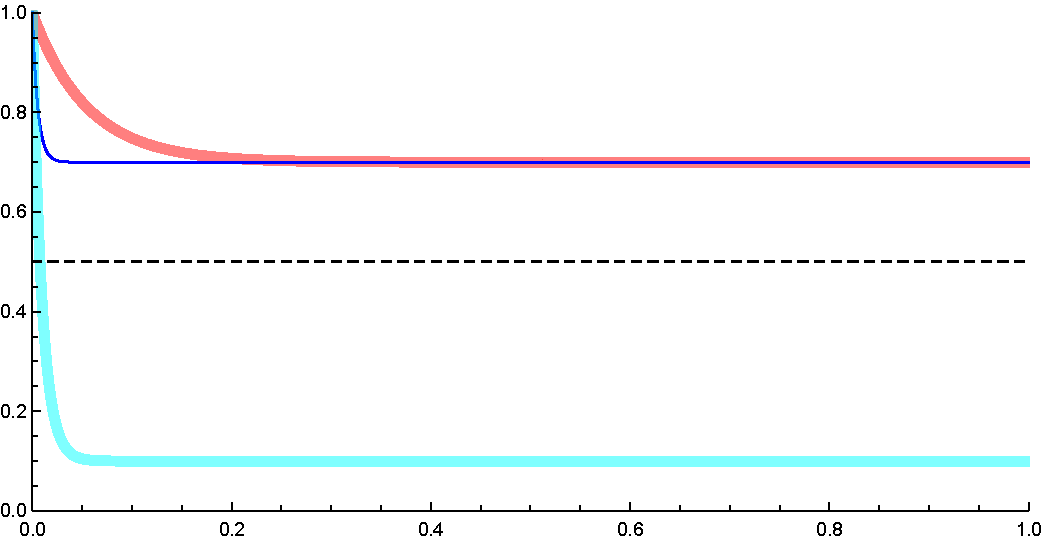
\includegraphics[width=5in]{./figures/broadening.eps}
	\caption{(a) A semi-infinite long strip subjected to an applied total strain $\e_0$. (b-f) The phase field $\phi$ at different strain levels}
	\label{fig: schematic}
\end{figure}
%
\begin{equation}
	\Delta d-\frac{d}{l^2}=\frac{g^\prime(d)}{2g_c l}\e:\C:\e.
\end{equation}
with $g(d) = (1-d)^2$ becomes
\begin{equation}
	d''-\frac{d}{l^2} = -\frac{E\e_0^2}{g_cl}(1-d)
\end{equation}
Let $\beta = \frac{E\e_0^2}{g_cl}$, $\alpha=\beta+\frac{1}{l^2}$. The general solution of 
\begin{equation}
	d''-\alpha d + \beta = 0
\end{equation}
is 
\begin{equation}
	d(x) = \frac{\beta}{\alpha} + C_1 e^{-\sqrt{\alpha}x} + C_2 e^{\sqrt{\alpha}x} 
\end{equation}
According to the boundary conditions
\begin{equation}
	d(0) = 1 \quad \text{and} \quad |d(x)| < \infty \quad \text{for} \quad x\in [0,\infty],
	\label{eq: bcs}
\end{equation}
we determine the constants to be $C_1=\frac{1}{1+\beta l^2}$ and $C_2=0$. Thus
\begin{equation}
	d(x) = \frac{\beta}{\alpha} + \frac{1}{1+\beta l^2} e^{-\sqrt{\alpha}x}.
\end{equation}

As an example, let $E = 5.0\times10^{-5}$, $g_c = 0.5$, $l = 1.0\times10^{-2}$. The plots of $d(x)$ at different strain levels are shown in Fig.~\ref{fig: ddistr}.

We still need to check the equilibrium of stress to be satisfied. We note that 
\begin{equation}
	\sigma = g(d) \C:\e
\end{equation}
with components $\sigma_{xx} = 0$, $\sigma_{xy} = 0$, and $\sigma_{yy} = (1-d(x))^2 E\e_0$. Then the equilibrium follows by substituting the stress into the equation $\nabla\cdot\sigma=0$.

\subsection{Load controlled}
Instead of applying displacement, we prescribe traction $\sigma_0$ at the top and button boundary. According to equilibrium equation, the only non-zero stress is $\sigma_{yy} = \sigma_0$. Then the governing equation of $d(x)$ is
\begin{equation}
	d''-\frac{d}{l^2} = -\frac{\sigma^2}{g_cl}\frac{g'(d)}{g(d)^2} = -\frac{\sigma^2}{g_clE}\frac{1}{(1-d)^3},
\end{equation}
or written as
\begin{equation}
	d''-\alpha d + \beta (1-d)^{-3} = 0
\end{equation}
with $\alpha=\frac{1}{l^2}$ and $\beta = \frac{\sigma^2}{g_clE}$. The boundary conditions are Eq.~\ref{eq: bcs}.


%%%%%%%%%%%%%%%%%%%%%%%%%%%%%%%%%%%%%%%%%%%%%%%%%%%%%%%%%%%%
%%%%%%%%%%%%%%%%%%%%%%%%%%%%%%%%%%%%%%%%%%%%%%%%%%%%%%%%%%%%
\newpage
\bibliographystyle{unsrt}
\bibliography{bib1}

\end{document}
